\section{Hardware Device}

Our prototype consists of a Google Glass Explorer Edition head-worn computing device, augmented with an infrared emitter that is mounted on the frame, pointing out in the direction of the wearer's view (Figure~\ref{fig:glass}). The IR emitter LED is mounted in an opaque hollow tube, that restricts the outgoing angle of illumination. The angle can be adjusted by moving the LED in or out of the tube.

Glass communicates a device id over the IR channel analogous to Patel's approach~\cite{patel_2-way_2003}. Target appliances have IR receivers and offer immediate visual feedback by toggling an LED whenever a valid id is received.

When users confirm that, further communication switches over to a ZigBee wireless network so that line of sight to the target is no longer needed.

In our prototype, Glass communicates over Bluetooth to an additional microcontroller PCB the user has to wear. This board marshals XBee to Bluetooth messages in both directions and also controls the IR LED mounted on the Glass frame. This architecture was mostly chosen for reasons of expediency. Future headmounted devices could clearly integrate IR emitters; the choice of local area wireless technology could also change . \bjoern{why not all bluetooth? There's probably a pairing/latency argument to be made here.} 


\subsection{Device Characterization}
We characterized the usable range and selection accuracy... (see Figure~\ref{fig:coverage} and Table~\ref{table:measurements}).
\bjoern{insert text from google doc here}


\begin{figure}[t]
\centering
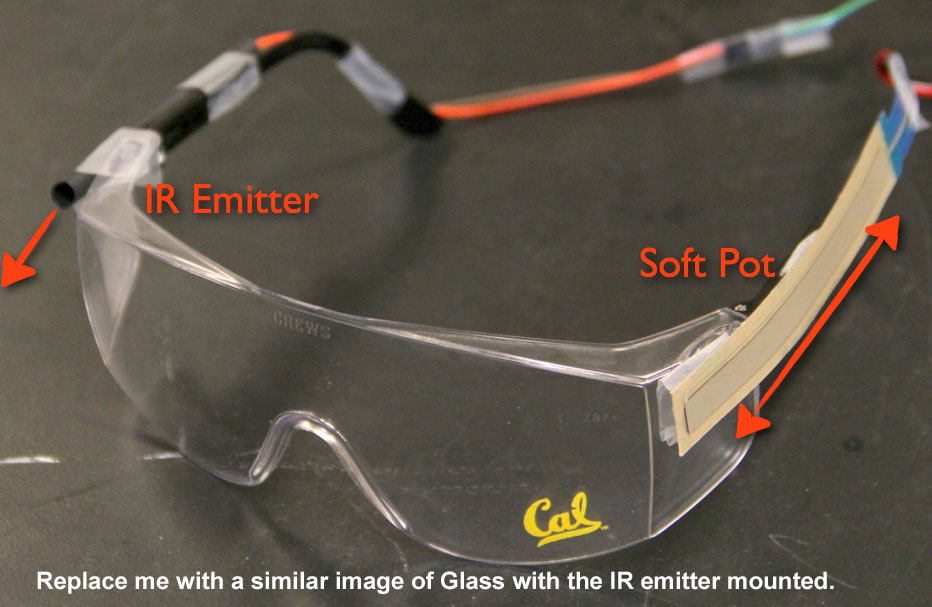
\includegraphics[width=1.0\columnwidth]{figures/glass-with-ir}
\caption{Our augmented Glass prototype has a frame-mounted infrared emitter.}
\label{fig:glass}
\end{figure}


\begin{figure}[t]
\centering
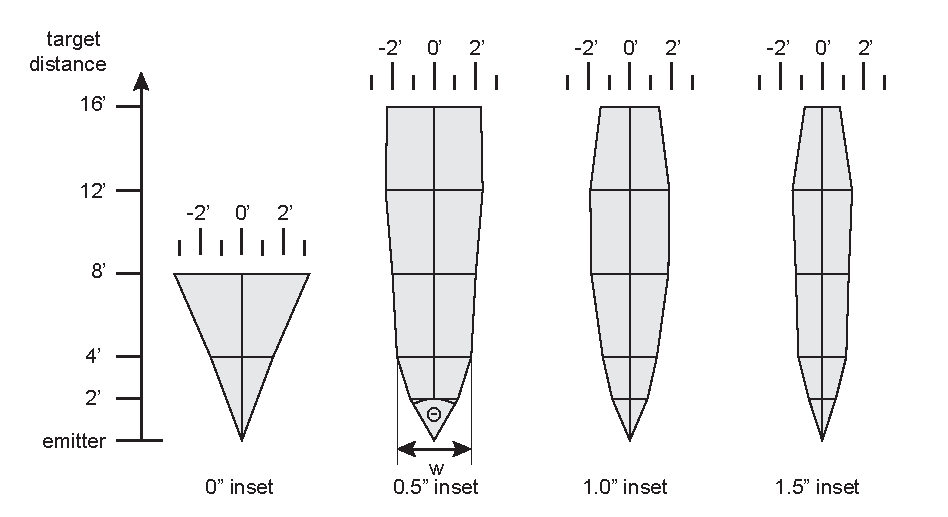
\includegraphics[width=1.0\columnwidth]{figures/glass-ir-coverage}
\caption{Our augmented Glass prototype has a frame-mounted infrared emitter.}
\label{fig:coverage}
\end{figure}

\begin{table}
    \begin{tabular}{l|lllll}
    distance/ depth & \ft2       & \ft4       & \ft8   & \ft{12}  & \ft{16}  \\ \hline
    \inch{0}                     & $74\degree$ & $78\degree$ & N/A  & N/A  & N/A  \\
  \inch{0.5}                   & $60\degree$ & $48\degree$     & $28\degree$ & $22\degree$ & $16\degree$ \\
    \inch{1.0}                     & $46\degree$     & $36\degree$     & $26\degree$ & $18\degree$ & $10\degree$ \\
    \inch{1.5}                   & $36\degree$     & $32\degree$     & $18\degree$ & $14\degree$ & $6\degree$  \\
    \end{tabular}
    \caption{Measured IR coverage angles $\Theta$ at different target distances and different depths of IR emitter inside shielding tube.}
    \label{table:measurements}
    
\end{table}